\begin{figure}[h]
	\centering
	\missingfigure{Komponentendiagramm}		
	\caption{Komponentendiagramm - A}
	\label{fig:komponentendiagramm-a}
\end{figure}

\begin{tcolorbox}
Die strukturelle Übersicht des zu entwickelnden Systems wird mittels Komponentendiagrammen modelliert. 
Auf jedes Diagramm muss eine textuelle Beschreibung (Fließtext mit Umbrüchen / Absätzen oder Tabelle) folgen, in der die Aufgaben der Subkomponenten beschrieben werden. 
\end{tcolorbox}

\section{App}

Die App ist in mehrere Komponenten aufgeteilt, von denen die meisten direkt die Java-Packages des Projektes darstellen. Ausnahmen sind die Actvities in der UI Komponente, die wir hier eintragen obwohl sie häufig nur eine Activity-Klasse umfassen, weil sie darüber hinaus mehrere XML Dateien und andere Resourcen nutzen.\\
Die meisten Anfragen der UI gehen an die Controller Klassen, die außerdem als Fassade zwischen Front- und Backend der App darstellen. Allerdings Kommuniziert die UI bei manuellen Uploads direkt mit der Meter Klasse, die in der Internal Komponente liegt.\\ 

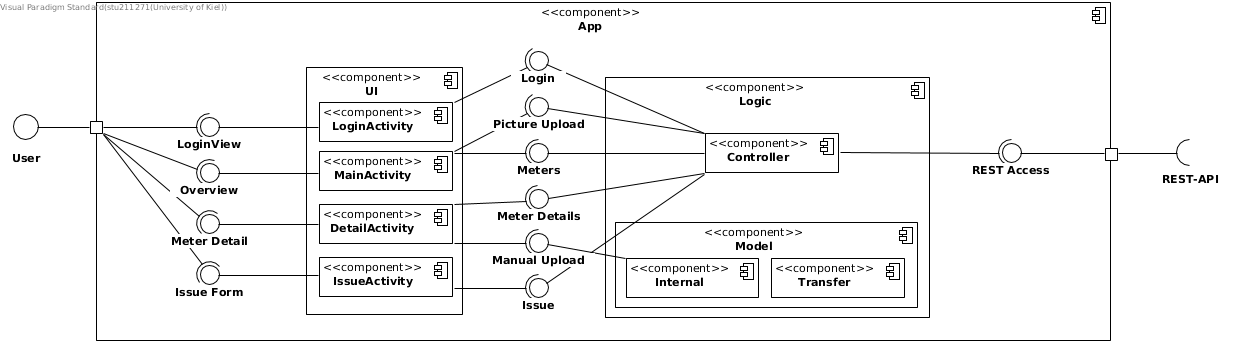
\includegraphics[scale=0.45]{img/diagrams/AppComponentDiagram} 